\subsection{Tools (Magnus)}\label{sec:tools}

First we present the tools used, complementing those in the IBM section (the mainframe, z/OS, DB2). Then we reflect on the advantages and disadvantages of each. 

The tools used in this project were given, and are seen in Fig \ref{fig:communication_external}. In short: The application is written in \textbf{Java}, and runs on a \textbf{z/OS} operating system on an \textbf{IBM mainframe}. The customer data is stored in a \textbf{DB2 database}, also in the mainframe. The user interacts with the application through a \textbf{web browser} e.g. Chrome. We chose to build the web pages with \textbf{JSP}.

\textbf{Why use Java?} Java has a vast set of libraries that makes implementation fast. Java runs slower than e.g. C, but has no buffer overflow. We have experience with Java from DTU course 02101. Eclipse offers Git tools for version control. Java is a language used on the Danske Bank IBM mainframe, so it is a valid real-life choice \cite{danskebank_java}.

 

\textbf{Why use JSP?} \textbf{J}ava\textbf{S}erver \textbf{P}ages is a technology that integrates Java code and HTML. This means we could apply our knowledge of Java when creating web pages. There are other popular technologies for building web pages, but as we have little experience with web development, JSP seemed like a good choice. We had to self-study some HTML, but as HTML the most popular markup language for web pages \cite{html_most_used}, this was good time investment.

\begin{figure}[H]
\centering
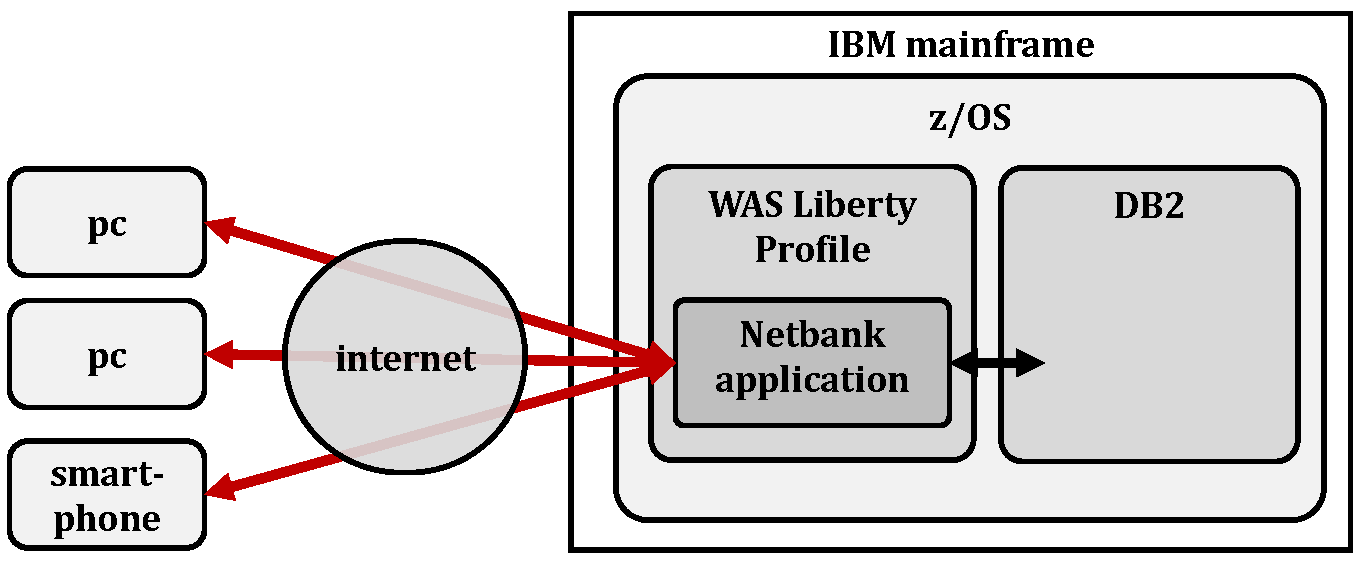
\includegraphics[width = 0.7\textwidth]{figures/communication1.pdf}
\caption{Commutation chart, when the application is running on the IBM Mainframe.}\label{fig:communication_external}
\end{figure}

